\documentclass[11pt]{beamer}
\usetheme{Goettingen}
\usepackage[utf8]{inputenc}
\usepackage{amsmath}
\usepackage{amsfonts}
\usepackage{amssymb}
\usepackage{graphicx}
\usepackage{hyperref}
\usepackage[hang,flushmargin]{footmisc}

\title{Equivariant Prediction of Tensorial Properties and Transfer Learning}
\author{Alex Heilman}
%\setbeamercovered{transparent} 
%\setbeamertemplate{navigation symbols}{} 
%\logo{} 
%\date{} 
\addtobeamertemplate{navigation symbols}{}{%
    \usebeamerfont{footline}%
    \usebeamercolor[fg]{footline}%
    \hspace{1em}%
    \insertframenumber/\inserttotalframenumber
}


\usepackage[style=authortitle,backend=bibtex]{biblatex}
\addbibresource{chgcnn.bib}

\newenvironment{boxed2}
    {\begin{center}
    \begin{tabular}{|p{0.95\textwidth}|}
    \hline\\
    }
    { 
    \\\\\hline
    \end{tabular} 
    \end{center}
    }


\renewbibmacro*{\tiny cite:title}{\tiny%
  \printtext[bibhyperref]{%
    \printfield[citetitle]{labeltitle}%
    \setunit{\space}%
    \printtext[parens]{\printdate}%
  }%
}

\begin{document}

\begin{frame}
\titlepage
\end{frame}

%\begin{frame}
%\tableofcontents
%\end{frame}

\begin{frame}{Overview}
$\bullet$ $J_z$ basis $\rightarrow Y_{\ell = 1}^m$ unit vectors

\medskip

$\bullet$  Clebsch-Gordon expansion for symmetric tensor spaces

\medskip

$\bullet$  Constructing symmetric, $SO(3)$ invariant, tensor subspaces

\medskip

$\bullet$  Equivariant networks and harmonics

\medskip

$\bullet$  Test results: pretraining and prediction
\end{frame}

\begin{frame}{$J_z$ Basis}
Recall $\ell=1$ spherical harmonics (with Racah normalization):
\begin{align*}
Y_1^{+1} &= -\frac{1}{\sqrt{2}}(x+iy)=\frac{1}{\sqrt{2}}\sin \phi e^{i\theta}\\
Y_1^{0}\ \ &= z = \cos \phi\\
Y_1^{-1} &= -\frac{1}{\sqrt{2}}(x-iy)=\frac{1}{\sqrt{2}}\sin \phi e^{-i\theta}
\end{align*}
\begin{center}
So, define $J_z$ basis:
$$
\begin{bmatrix}
a_+ \\
a_0 \\
a_-
\end{bmatrix}=\begin{bmatrix}
-\frac{1}{\sqrt{2}} & -\frac{i}{\sqrt{2}} & 0\\
 0 & 0 & 1\\
-\frac{1}{\sqrt{2}} & +\frac{i}{\sqrt{2}} & 0\\
\end{bmatrix}\begin{bmatrix}
x \\
y \\
z
\end{bmatrix}
$$
so that $\hat{n}=a_+ Y_1^1 + a_0 Y_1^0 + a_- Y_1^{-1}$
\end{center}
\end{frame}
\begin{frame}{Clebsch-Gordon Expansion}
Build larger spherical harmonic tensors with CG expansion:
$$
Y_{\ell_1}^{m_1}\otimes Y_{\ell_2}^{m_2} = \sum_{L=-|\ell_1-\ell_2|}^{\ell_1+\ell_2}\sum_{M=-L}^{L}c_{\ell_1 0 \ell_2 0}^{L0}c_{\ell_1 m_1 \ell_2 m_2}^{LM}Y_{L}^M
$$
where $Y_{L}$ represents a $2L+1$ dimensional symmetric tensor space of rank $L$. 

We use this as a relation between symmetric tensor's $J_z$ basis components and higher order spherical harmonic tensors. 

$$ 
T^{(n)} = a_{\underbrace{\alpha\beta...}_n}\big(Y_1^\alpha \otimes Y_1^\beta\otimes ... \big)\ \  \Rightarrow\ \  y_\ell^m Y_L^M
$$

\begin{center}
But, what about asymmetric tensors?
\end{center}
\end{frame}
\begin{frame}{$SO(3)$ Invariant Tensor Subspaces}
We can always reduce an arbitrary tensor $T$ that transforms under a transformation as:
$$
T_{x_1x_2...x_n}\rightarrow T_{x'_1x'_2...x_n'}=R_{x_1'}^{x_1} R_{x_2'}^{x_2} R_{x_3'}^{x_3}T_{x_1x_2...x_n},
$$
into a set of irreducible (but not necessarily unique) symmetric, $SO(3)$ invariant subtensors:
$$
\lbrace h^{(\ell)}\rbrace \rightarrow \lbrace h'^{(\ell)}\rbrace = \lbrace \mathcal{D}^{\ell}(R) h^{(\ell)}\rbrace
$$

This decomposition can be constructed by consecutive decomposition with respect to $GL$ and then $O$ and $SL$
$$
SO= SL\cap O \subset GL
$$
\end{frame}
\begin{frame}{$GL$ Decomposition}
$\bullet$ Decompositions under general linear group $GL$ are simultaneous with decompositions under symmetric group $S$ (\textit{Schur-Weyl Duality})

\medskip

$\bullet$ Irreducible representations of symmetric group are diagramatically described by Young diagrams.

\begin{center}
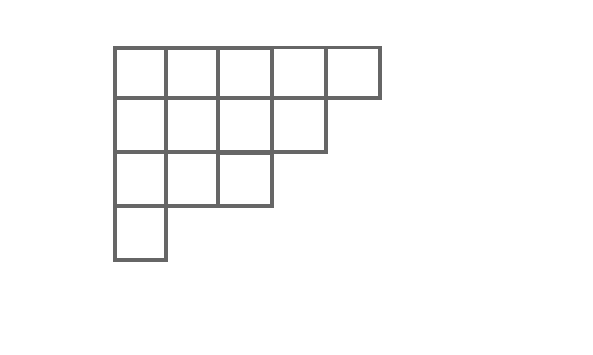
\includegraphics[scale=0.6]{youngdiagram-ex.pdf}
\end{center}
Young diagrams  are said to be of some shape $\lambda:(\lambda_1,\lambda_2,...,\lambda_k)$, where $\lambda_i$ refers to the depth of row $i$ and $\lambda_{i+1}\leq\lambda_i\leq\lambda_{i-1}$. Above: $(5,4,3,1)$
\end{frame}
\begin{frame}{$GL$ Decomposition cont.}
We can then form a set of Young tableaux from diagrams by filling in the boxes from a set of ordered indices $\lbrace x_1,x_2,...,x_k\rbrace$ corresponding to tensor components $T^{x_1x_2...x_k}$. 
\begin{center}
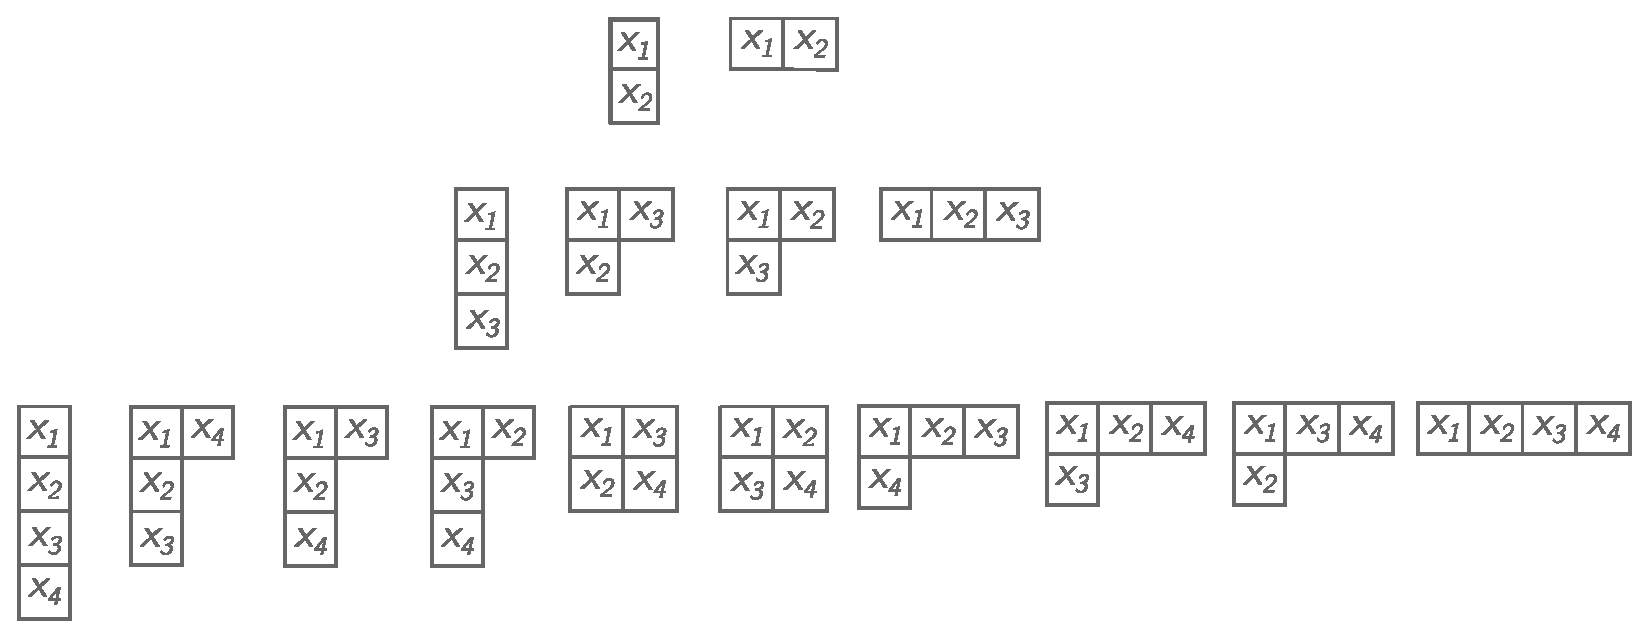
\includegraphics[scale=0.3]{youngtableaux-ex.pdf}
\end{center}
A standard tableu is one filled with indices $x_i$ (without repeats) with entries increasing in index $i$ down each column and across (to the right) rows.
\end{frame}

\begin{frame}{$GL$ Decomposition cont.}
Each of these standard tableaux correspond to an invariant subspace under $S_k$.

\medskip

These invariant subspaces may be constructed by correspond products of symmetrizers $s$ and antisymmetrizers $a$:
$$
s_{\lambda} = \prod_{\mathcal{I}\in \text{Cols}(\lambda)}\mathcal{S}(\mathcal{I})
$$
$$
a_{\lambda} = \prod_{\mathcal{I}\in \text{Rows}(\lambda)}\mathcal{A}(\mathcal{I})
$$
\begin{center}
where $\mathcal{S}$ and $\mathcal{A}$ act component-wise as:
\end{center}
$$
\big[\mathcal{S}(\mathcal{I})T\big]_{ijk...}= \sum_{\sigma_{\mathcal{I}}}T_{\sigma_{\mathcal{I}}(ijk...)}
$$
$$
\big[\mathcal{A}(\mathcal{I})T\big]_{ijk...}= \sum_{\sigma_{\mathcal{I}}}\text{sgn}(\sigma_{\mathcal{I}})T_{\sigma_{\mathcal{I}}(ijk...)}
$$
\end{frame}

\begin{frame}{$O$ Decomposition}
Orthogonal group $O$, preserves inner product between vectors $<\cdot , \cdot >$. defined by means of a metric tensor $g_{ij}$ , which transforms as a second rank tensor under some transformation $R$ as:
$$
g_{x_1x_2}\rightarrow g_{x'_1x_2'} = R_{x_1'}^{x_1} R_{x_2'}^{x_2}g_{x_1x_2}
$$
Contractions of arbitrary tensors $T$ with $g_{ij}$ are invariant under $O$.

\medskip

For example, consider the rank-3 covariant $T^{ijk}$:
$$
g_{i'j'}T^{i'j'k'} = S^{k'}= R_{i'}^{i} R_{j'}^{j} g_{ij}R_{i}^{i'} R_{j}^{j'}R_k^{k'}T^{ijk} = R_k^{k'} S^k
$$
so that $S$ acts like an invariant vector subspace under $O$.
\end{frame}
\begin{frame}{$SL$ Decomposition}
Special linear group $SL$ of transformations is defined as invertible linear transformations with determinant equal to positive one.

\medskip

Under $SL$, orientation and volume are preserved, where volume is defined as the contraction of a tensor with the fully antisymmetric tensor $\epsilon_{ijk}$, which transforms under $R\in GL(3)$ as:
$$
\epsilon_{x_1x_2x_3} \rightarrow\epsilon_{x_1'x_2'x_3'} =\text{det}(R) R_{x_1'}^{x_1} R_{x_2'}^{x_2}R_{x_3'}^{x_3}\epsilon_{x_1x_2x_3} 
$$
Similar to the case of $g_{ij}$ in $O$, contractions with $\epsilon_{ijk}$ of arbitrary tensors yield $SL$ invariant subspaces.
\end{frame}

\begin{frame}{$SO(3)$ Decompositions}
\small
In $SO(3)$, we may use all of the above (Young, $g_{ij}$, $\epsilon_{ijk}$):

\medskip

$\bullet$ Young symmetrizers return a set of tensors of known symmetries (under index permutation).

\medskip


$\bullet$ Contractions with $g_{ij}$ along antisymmetric pairs of indices vanish.

\medskip

$\bullet$ Contractions with $\epsilon_{ij}$ along symmetric sets of indices vanish.

\vspace{1cm}

These may all be used together to decompose an arbitrary tensor into a set of symmetric, $SO(3)$ invariant, symmetric tensor subspaces. These then may be related to harmonic coefficients by way of the CG expansion from the $J_z$ basis given before.
\end{frame}
\begin{frame}{Example: Piezoelectric Tensors}

The piezoelectric strain components $d_{ijk}$ are symmetric under $i,j$ so that:
$$
d_{ijk}=d_{jik}
$$
according to this symmetry, we see all Young tableaux but the following must disappear:
\begin{center}
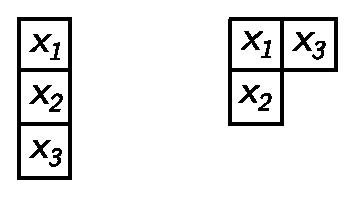
\includegraphics[scale=0.7]{piezo_young.pdf}
\end{center}defined component-wise (using the defining symmetry):
\begin{align*}
S_{ijk}&=\frac{1}{3}\big(d_{ijk}+d_{jki}+d_{ikj}\big)\\
A_{ijk}&=\frac{1}{3}\big(2d_{ijk}-d_{jki}-d_{ikj}\big)\\
\end{align*}
\end{frame}
\begin{frame}{Example: Piezoelectric Tensors}
This may be derived as (adopting the convention of symmetrization before antisymmetrization):
\begin{center}\small
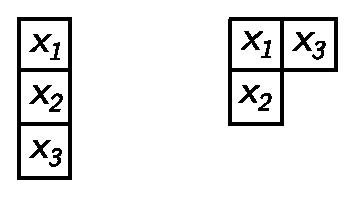
\includegraphics[scale=0.5]{piezo_young.pdf}
$$
\mathcal{S}(ijk)\quad\quad \mathcal{A}(ij)\mathcal{S}(ik)
$$
\begin{align*}
\mathcal{S}(ijk)d_{ijk}& =d_{ijk}+d_{ikj}+d_{kji}+d_{jki}+d_{kij}+d_{kji}\\
&=2( d_{ijk}+d_{ikj}+d_{kji})\\
\\
\mathcal{A}(ik)\mathcal{S}(ij)d_{ijk}& =\mathcal{A}(ij)(d_{ijk}+d_{jik})\\
&=d_{ijk}-d_{kji}+d_{jik}-d_{jki}\\
&= 2d_{ijk}-d_{kji}-d_{jki}
\end{align*}
\end{center}
Where the respective normalization coefficients (neglected here) may be derived from the diagram's shape via the hook-length formula.
\end{frame}
\begin{frame}{Example: Piezoelectric Tensors}
\begin{center}
Further decompose $A$ into the trace vector $v_i$:
$$
v^i =g_{jk}A^{ijk}
$$

and the traceless, symmetric tensor $b_{ij}$:
$$
b_{ij}=\frac{1}{2}\big(\epsilon_{i}^{mk}A_{mkj}+\epsilon_{j}^{mk}A_{mki}\big)
$$
\end{center}
\end{frame}
\begin{frame}{$SO(3)$ Equivariant Networks}
An $SO(3)$ equivariant network is a neural network  satisfying:
$$
f(\lbrace \mathcal{D}^{\ell_1}(R)h_{(\ell_1)}\rbrace) = \lbrace\mathcal{D}^{\ell_2}(R) h'_{(\ell_2)}\rbrace \quad\quad \forall R\in SO(3)
$$
This can be accomplished by associating hidden features $V$  and filters $F$ with spherical harmonics defining convolution as their tensor product:
$$
\mathcal{L}^{\ell_o}_{acm_o}\big(\vec{r}_a,V_{acm_i}^{\ell_i}\big) = \sum_{m_f,m_i}c_{\ell_im_i\ell_fm_f}^{\ell_o m_o}\sum_{b}F^{\ell_f\ell_i}_{cm_f}(r_{ab})V_{bcm_i}^{\ell_i}
$$
The important thing to note here is that these networks naturally yield coefficients of spherical harmonic tensors.
\end{frame}

\begin{frame}{General Model Architecture}
\begin{center}
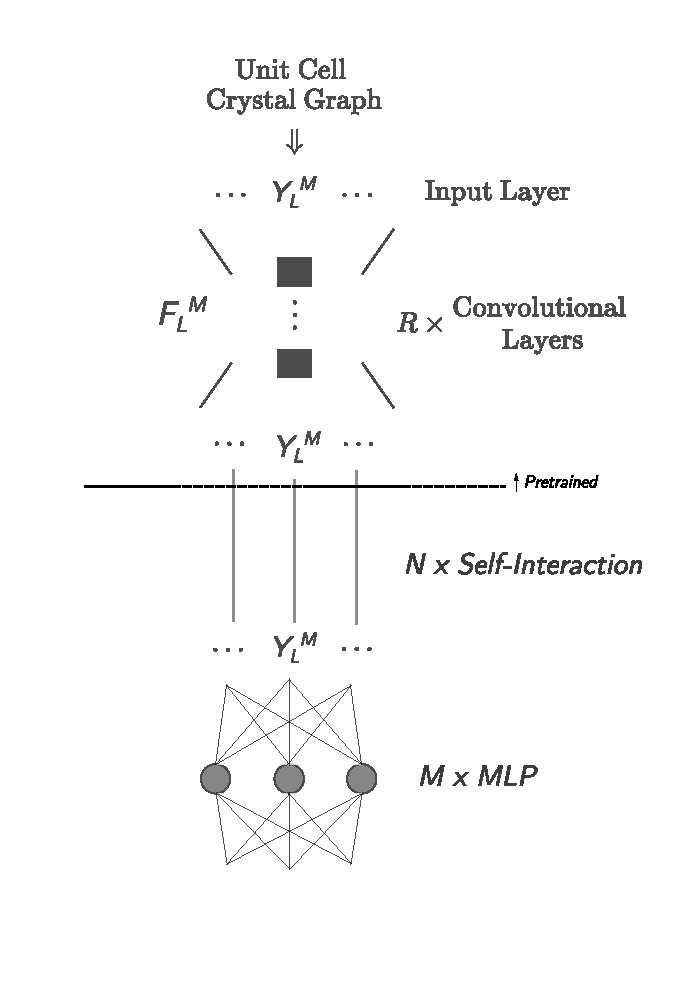
\includegraphics[scale=0.5]{architecture.pdf}
\end{center}
\end{frame}

\begin{frame}{Training Progressions}
Pretraining consisted of a funnel-down approach where the first graph layers were first trained on the largest set, then trained on the second largest, etc.

\vspace{1cm}

Here, this corresponds to the progression:
$$
\text{Band Gap} \rightarrow \text{Elasticity} \rightarrow \text{Dielectric} \rightarrow \text{Piezoelectric}
$$

This progression is compared to blind training on each dataset individually
\end{frame}

\begin{frame}{Results}

\begin{tabular}{c|ccc}
& Elasticity (10,829)& Dielectric & Piezoelectric\\
Model & MAE (log(GPA)) & MAE  & MAE (GPA$^{-1}$) \\
\hline
Blind & 7.387 & 4.818 & 0.170\\
Pretrain & 7.274 &4.525 &0.170\\
\end{tabular}

\vspace{0.8cm}

The low impact of pretraining may be due to several factors:

\medskip

$\bullet$ Lack of shared domain-relevance in graph layers

$\bullet$ Lack of overlap in datasets (unlikely)

$\bullet$ Lack of overlap in filters for different $\ell$ order targets

\end{frame}

\end{document}